\clearpage

\section{Freay and Hinton: Bits-back with arithmetic coding}\label{sec:arithmeticbitsback}\index{bits-back}

\begin{notebox}
\textbf{Paper: } \fullcite{DBLP:journals/cj/FreyH97}

\hfill Notes taken: 4/6/2021 \index{June 2021}
\end{notebox}

\begin{notebox}
\tldr In a mixture model it may be difficult to directly evaluate $p(\rvx)$ so that you can transmit $\rvx$ by entropy encoder. You may hence want to use the prior $p(\rvy)$ and the conditionals $p(\rvx | \rvy)$ to transmit the message $(\rvy, \rvx)$.
However, for each $\vx$, there are multiple different codewords with different length $l(\vy, \vx)$ depending on the choice of $\vy$ and hence the conditional $p(\vx | \vy)$.
A natural choice is the shortest such codeword.
They show and demonstrate on experiments, that you can do better (and theoreticaly get to the optimal expected transmission length $- \logb p(\vx)$) in a bits-back coding scheme in which the encoder uses some auxiliary data to sample $\vy$ that will be transmitted determining also the corresponding $p(\vx | \vy)$ used for encoding $\vx$.
Since the decoder can recover these auxiliary data it gets some bits for free without them being directly included in the transmission. These are the bits back that reduce the effective transmission length.
\end{notebox}


\subsection{Intro}

A \iterm{source code} uses as \iterm{source model} to map each input symbol to a unique \iterm{codeword}.
There are two principal source models:
\textbf{one-to-one} where each symbol is mapped to a single codeword;
\textbf{one-to-many} where each symbol is mapped to a distribution across multiple codewords.
One-to-many source models arrise naturally in many domains such as in mixture distributions
\begin{align}
\rvx \in \sX \sim p(\rvx) = \sum_y p(\rvy) p(\rvx \vert \rvy) \enspace .
\end{align}.

For example for the mixture of Gaussian in \figref{fig:Frey1997} the optimal one-to-one model uses codewords with length given by the information content of the symbols $l(\rvx) = h(\rvx) = -\logb p(\rvx)$.

\begin{figure}[h]
\centering
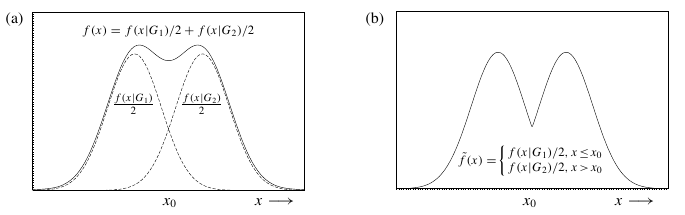
\includegraphics[width=0.8\textwidth]{Pics/Frey1997.png}
\caption{Mixture of two Guassians.}
\label{fig:Frey1997}
\end{figure}

In one-to-many model, we have for each symbol $\vx$ two possible codewords: one given by $G_1$ the other by $G_2$ with the lengths given by $h_{\vx|\vy}(\vx) = -\logb p(\rvx | \rvy = \ry), \ry \in \{1, 2\}$ respecitvely.
Assuming the prior $p(\rvy = 1) = p(\rvy = 2) = 0.5$ we also have $h_{\vy}(1) = h_{\vy}(2) = - \logb 0.5 = 1$ bit to communicate $\rvy$ and hence the identity of the conditional distribution.

A natural choice is to always pick the shorter of the two codewords for $\vx$. This corresponds to a distribution in (b) in \figref{fig:Frey1997} which is clearly suboptimal (gives longer codes then the one-to-one) around $\vx_0$.

\begin{notebox}
Here they show how stochastic one-to-many model relying on the \iterm{bits-back} idea can achieve same rates as the one-to-one scheme.
\end{notebox}

\paragraph{Running example: } We want to encode a symbol $\vx$ that is twice as likely under $G_1$ then $G_2$ so that it requires 2 and 3 bits respectively under the two distributions (that is $p(\vx | \rvy = 1) = 1/4$ and $p(\vx | \rvy = 2) = 1/8$).
With 1 bit to specify the $\rvy$ and hence the conditional distribution we get the total lenght of 3 and 4 bits for the two-level code.
We now have the following options:
\begin{enumerate}[noitemsep, topsep=0pt]
\item picking alwyas the shorter code gives expected length of 3 bits;
\item picking between the two codes equally often (according to the prior $p(\rvy)$) gives expected length of 3.5 bits;
\item use bits-back to get the expected length 2.5 bits.
\end{enumerate}

\begin{notebox}
\paragraph{This is the bits-back idea:}\index{bits-back}
Instead of picking always the shortest codeoword or pick equally often amongst the codeword in the one-to-many setup, you will be picking $\vy \in {1, 2}$ randomly according to some probability $q(\rvy | \rvx)$.
However, to select (sample) $\rvy$ you will use some random sampler based on transorming some auxiliary data $\rvz$ into the samles $\rvy \sim q(\rvy)$.
A trivial example for univariate case is the inverse CDF sampling starting from uniform $\rvz$ or, as they suggest here, the arithmetic decoding which can produce vectorial $\rvy$ starting from a random binary sequence $\rvz$.
Once you sampled $\vy$ you will encode it using $p(\rvy)$ and concatenate with the encoding of $\vx$ using the corresponding $p(\vx | \vy)$.
The message you transmit thus has length $l(\vx, \vy) = - \logb p(\vx | \vy) - \logb p(\vy)$.

The reciever has access to the encoding models $p(\rvy), p(\rvx | \rvy)$ and it 
can thus easily decode the symbols $\rvx$ and $\rvy$ from the codewords $C(\rvx, \rvy)$.
However, it also has access to the sampling distribution $q(\rvy)$ and the algirithm the encoder uses to sample $\rvy$ by transforming $\rvz$.
It can thus reverse this operation (so the transformation must be one-to-one) and recover $\rvz$ at no additional communication cost - these are the `bits-back'.
If $\rvz$ contains some useful information, these `bits-back' essentially reduce the \iterm{effective message length}.
\end{notebox}

In our \textbf{running example} lets imagine $\rvz \in {a, b}$ with $p(\rvz=a)=p(\rvz=b)=0.5$.
Then once we recover $\rvz$ we have communicated $h_{\rvz}(\vz) = - \logb 0.5 = 1$ bit of information at no cost and so the \textbf{expected effective length is $3.5 - 1 = 2.5$ bits}.

How many bits can be recovered is a function of the probability distribution $q(\rvy | \rvx)$.

The \textbf{average code length} for a symol $\vx$ is
\begin{align}
\mathcal{E}(\vx) = \sum_y q(\vy | \vx) l(\vx, \vy) \enspace .
\end{align}
Here $l(\vx, \vy) = - \logb p(\vx | \vy) - \logb p(\vy)$ are the different lengths using different conditionals to encode $\vx$ depending on the choice of $\vy$.

The average information content (the entropy) of the selecting distribution
\begin{align}
\mathcal{H}(\vx) = - \sum_y q(\vy | \vx) \logb q(\vy | \vx)
\end{align}
are \textbf{the average bits back we can recover} for this symbol $\rvx$ when choosing $\vy$ according to $q(\rvy | \vx)$.

\begin{notebox}[colback=yellow!5]
For this you need to recall that $q(\vy | \vx)$ is the coding model which is used to get from the auxiliary $\vz$ to $\vy$ - $\vz$ is the codeword for $y$ under the coding model $q(\vy | \vx)$ with length $l(\vy) = - \log q(\vy | \vx)$ are these are the bits we get back.
So the above example of using inverse CDF is probably nonsense.
\end{notebox}


The average effective codeword length of symbol $\vx$ is the difference between the two above
\begin{align}
\mathcal{F}(\vx) = \mathcal{E}(\vx) - \mathcal{H}(\vx) \enspace .
\end{align}
This is also called the \textbf{\iterm{free energy}} - same concept known from statistical physics.

Next comes the question what $q(\rvy | \vx)$ shall be.
They claim it shall be the Boltzman distribution based on the codeword lengths
\begin{align}
q^*(\vy | \vx) = \frac{2^{-l(\vx, \vy)}}{\sum_{\vy'} 2^{-l(\vx, \vy')}}
\end{align}

\begin{proof}[My proof for Boltzman:]
\begin{align*}
\mathcal{F^*}(\vx) & = \mathcal{E^*}(\vx) - \mathcal{H^*}(\vx)
= \sum_y q^*(\vy | \vx) l(\vx, \vy) + \sum_y q^*(\vy | \vx) \logb q^*(\vy | \vx) \\
& = \sum_y \frac{2^{-l(\rvx, \rvy)}}{\sum_{y'} 2^{-l(\rvx, \rvy')}} \left[l(\rvx, \rvy) + \logb \frac{2^{-l(\rvx, \rvy)}}{\sum_{y'} 2^{-l(\rvx, \rvy')}}\right] 
= l(\rvx, \rvy) - l(\rvx, \rvy) - \logb \sum_{y'} 2^{-l(\rvx, \rvy')} \\
& = - \logb \sum_{y'} 2^{-l(\rvx, \rvy')} = 
- \logb \sum_{y'} 2^{\logb p(\vx, \vy)} =
- \logb \sum_{y'} p(\vx, \vy) = - \logb p(\vx)
\end{align*}
The Boltzman brings the free energy to the same lengths as if one-to-one code with $p(\rvx)$ were used so it is optimal.
\end{proof}

\begin{notebox}[colback=yellow!5]
I'd think it shall be the posterior $p(\vy \vert \vx) = p(\vy)p(\vx | \vy) / p(\vx)$.

\begin{proof}[My proof for posterior:]
\begin{align*}
\mathcal{F^*}(\vx) & = \mathcal{E^*}(\vx) - \mathcal{H^*}(\vx)
= \sum_y p(\vy | \vx) l(\vx, \vy) + \sum_y p(\vy | \vx) \logb p(\vy | \vx) \\
& = \sum_y p(\vy | \vx) \left[- \logb p(\vx, \vy) + \logb p(\vy | \vx)\right]
= \sum_y p(\vy | \vx) \left[- \logb p(\vx) \right] = - \logb p(\vx)
\end{align*}
The posterior brings the free energy to the same lengths as if one-to-one code with $p(\rvx)$ were used so it is also optimal.
\end{proof}

Does this mean that the Boltzman and the posterior distributions are the same?

\begin{align*}
q^*(\vy | \vx) & = \frac{2^{-l(\vx, \vy)}}{\sum_{\vy'} 2^{-l(\vx, \vy')}}
= \frac{2^{\logb p(\vx, \vy)}}{\sum_{\vy'} 2^{\logb p(\vx, \vy')}} \nn
& = \frac{p(\vx, \vy)}{\sum_{\vy'} p(\vx, \vy')} = \frac{p(\vx, \vy)}{p(\vx)} = p(\vy | \vx)
\end{align*}
So Boltzman baseded on the codeword lengths and the posterior are indeed one and the same thing!
\end{notebox}

% $p(\rvy \vert \rvx) p(\rvx) = p(\rvx , \rvy)$ so if we use this to get the codewords we get the lengths $l(\rvx, \rvy) = - \logb p(\rvx , \rvy)$.
% Plug this into the free energy
% \begin{align*}
% \mathcal{F(\rvx)} & = \mathcal{E(\rvx)} - \mathcal{H(\rvx)} = \sum_y p(\rvy | \rvx) l(\rvx, \rvy) + \sum_y p(\rvy | \rvx) \logb p(\rvy | \rvx) \\
% & = \sum_y p(\rvy | \rvx) \left[- \logb p(\rvx, \rvy) + \logb p(\rvy | \rvx)\right]
% = \sum_y p(\rvy | \rvx) \left[- \logb p(\rvx) \right] = - \logb p(\rvx)
% \end{align*}
% and we get this is equal to the optimal codelength for the one-to-one code based on $p(\rvx)$.
% \end{proof}

In our \textbf{running example} we use the result for the optimal free energy
$\mathcal{F^*}(\vx) = - \logb \sum_{y'} 2^{-l(\rvx, \rvy')}$ with the length
$l(\vx, 1) = 3$ bits and $l(\vx, 2) = 4$ bits we get
$\mathcal{F^*}(\vx) = - \logb (2^{-3} + 2^{-4}) = 2.415$ bits.
This is shorter (better) then the naive sampling used above with $q(\rvy | \vx) = 0.5$ which gave 2.5 bits.

\begin{notebox}
Alternative ways to write the free energy
\begin{align*}
\mathcal{F}(\vx) & = \mathcal{E}(\vx) - \mathcal{H}(\vx)
= \sum_y q(\vy | \vx) l(\vx, \vy) + \sum_y q(\vy | \vx) \logb q(\vy | \vx) \\
& = \sum_y q(\vy | \vx) \logb 2^{l(\vx, \vy)} + \sum_y q(\vy | \vx) \logb q(\vy | \vx) \\
& = \sum_y q(\vy | \vx) \logb \frac{ q(\vy | \vx)}{2^{-l(\vx, \vy)}}
= \sum_y q(\vy | \vx) \logb \frac{ q(\vy | \vx)}{p(\vx, \vy)} \\
& = \sum_y q(\vy | \vx) \logb \frac{ q(\vy | \vx)}{p(\vy | \vx) p(\vx)} 
= \sum_y q(\vy | \vx) \logb \frac{ q(\vy | \vx)}{p(\vy | \vx)}
- \sum_y q(\vy | \vx) \logb p(\vx)
\enspace .
\end{align*}

Here we are quickly getting to ELBO!
Take the expected free energy
\begin{align}\label{eq:Frey1997_elbo}
\E_{p(\rvx)} \mathcal{F}(\rvx)
& = \sum_x \sum_y p(\rvx) q(\vy | \rvx) \logb \frac{ q(\vy | \vx)}{p(\vy | \rvx)}
- \sum_x \sum_y p(\vx) q(\vy | \vx) \logb p(\vx) \nn
& = \KL(q(\rvy | \rvx) || p(\rvy | \rvx)) - \E_{p(\rvx)} \logb p(\rvx) = - ELBO
\end{align}
\end{notebox}

How much do we suffer from not using the Boltzman (posterior) $q^*(\vy | \vx) = p(\rvy| \vx)$ but some other distribution $q(\vy | \vx)$ to sample $\rvy$? 
Its the difference in the free energies:
\begin{align*}
\mathcal{F}(\vx) - \mathcal{F^*}(\vx) 
& = \sum_y q(\vy | \vx) l(\vx, \vy) + \sum_y q(\vy | \vx) \logb q(\vy | \vx) + \logb p(\vx) \nn
& = \sum_y q(\vy | \vx) \logb \frac{q(\vy | \vx) p(\vx)}{2^{-l(\vx, \vy)}}
= \sum_y q(\vy | \vx) \logb \frac{q(\vy | \vx) p(\vx)}{p(\vx, \vy)}
= \sum_y q(\vy | \vx) \logb \frac{q(\vy | \vx)}{p(\vy | \vx)}
\end{align*}
This is the KL divergence between the sampling distribution $q(\vy | \vx)$ and the optimal Boltzman or posterior distribution $p(\vy | \vx) = q^*(\vy | \vx)$.


\subsection{Bits-back coding algorithm}

If $\rvy$ is not simply two-valued or diadic (powers of two) variable, they propose to use arithmetic coding as the $f : \rvz \to \rvy$ algorithm.
I don't really see how that

\subsection{Link to maximum likelihood estimation}

In the maximum likelihood approach (see section \ref{sec:thoughts}) the cost we minimize is the length of codes $c(\vx) = - \logb p_{\vphi}(\vx) = - \logb \sum_\vy p_{\vphi}(\vx, \vy)$.

\begin{notebox}[colback=yellow!5]
In section \ref{sec:thoughts} we used $p(\vx | \vtheta)$ which I here call $p_{\vphi}(\vx)$ cause I use $\vtheta$ already.
\end{notebox}

For each pair $\vx, \vy$ we can use codeword with length $l(\vx, \vy) = -\logb p_{\vphi}(\vx, \vy)$ so that the maximum likelihood cost is $c(\vx) = -\logb \sum_\vy  2^{- l(\vx, \vy)} = \mathcal{F^*}(\vx)$.
\begin{notebox}
Maximum-likelihood cost is thus equal to the cost of optimal bits-back coding.
\end{notebox}

When we do not use the optimal $q(\rvy | \vx)$ then we get the ELBO equivalence in equation \eqref{eq:Frey1997_elbo}.

\subsection{Experiments}

Modelling binary data vectors $\rvx$ assuming these are produced by a set of hidden binary causes $\rvy$.
The model can produce codeword for each pair of these with length $l(\vx, \vy)$ (not restricted to be integer length here) so that $\sum_{\vx, \vy} 2^{-l(\vx, \vy)} \leq 1$.

\begin{notebox}[colback=yellow!5]
The above is called \iterm{Kraft inequality} and is a standard result in coding theory.
My translation is the following: if you always use the optimal length $l^*(\vx, \vy) = - \logb p(\vx, \vy)$ then it would be an quality $\sum_{\vx, \vy} 2^{-l(\vx, \vy)} = \sum_{\vx, \vy} p(\vx, \vy) = 1$.
But because you allow for some lengths being inefficient and therefore longer $l(\vx, \vy) \geq l^*(\vx, \vy)$ as if the corresponing $p(\vx, \vy)$ were somewhat smaller the result is the $\leq 1$.
\end{notebox}

The binary vector $\rvx$ contains $n_{\rvx}$ bits (lenght of the binary string); $\rvy$ contains $n_{\rvy}$ bits.
Together this creates $2^{n_{\rvx} + n_{\rvy}}$ possible messages, each with its own probability mass that needs to be established before encoding.

They use Bayesian network to get these probabilities.
Let $\vs = (\vy, \vx)$ and use the standard product rule of probability for the vector $p(\vs) = p(\evs_1) \prod_{i=2}^{n_{\rvx} + n_{\rvy}} p(\evs_i | \evs_{i-1}, \ldots, \evs_1)$.
They model each probability as a sigmoid $p(\evs_i | \evs_{<i}) = \sigmoid(\theta_i + \sum_{j < i} \theta_{ij}\evs_j)$, where they will learn the parameters $\vtheta$.

Furthermore they put some of the $\theta_{ij} = 0$ and use it tu create a hierarchy between the elements of the vector $\rvy$ essentially transforming it to a two layer binary cause $\rvy = (\rvc, \rvz)$ composed of two binary vectors with total length $n_{\rvy}$.
The lowest layer is modelled as a product distribution $p(\rvc) = p(\rvc_1)p(\rvc_2)p(\rvc_3) = p(\rvs_1)p(\rvs_2)p(\rvs_3)$ (product goes on depending on how many elements $\rvc$ has, in figure \ref{fig:Frey1997_2} it has 3).


\begin{figure}[h]
\centering
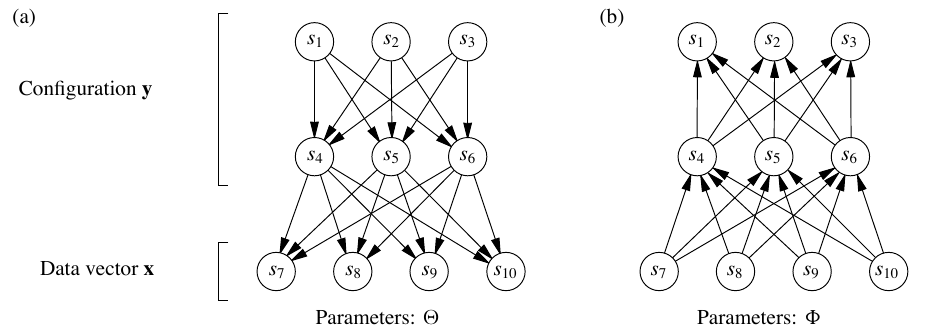
\includegraphics[width=0.8\textwidth]{Pics/Frey1997_2.png}
\caption{Bayesian network with two level hidden cuases.}
\label{fig:Frey1997_2}
\end{figure}

We can now encode any message $\vs = (\vy, \vx)$ by encodeing each $\vs_i$ by its probabiliy given by the Bayes net.

Given $\vx$ we would preferably want to pick $\vy$ according to the Boltzman which can also be written as $q^*(\rvy | \vx) = p(\vx, \vy) / \sum_\rvy p(\vx, \vy)$.
The sum in the denominator will have $2^{n_\rvy}$ terms which is clearly not tractable (or not reasonably) for any high dimensional $\rvy$ so using the Boltzman directly (the posterior) to pick the $\rvy$ is imposible.

Picking the shortest code is also expensive cause it would have to search among the $2^{n_\rvy}$ codewords based on $p(\vx | \vy)$ exhaustively.

Instead of the intractable $q^*(\rvy | \rvx)$ they will therefore use $q_{\vphi}(\rvy | \rvx)$ with the probabilities given by the reversed network given in figure \ref{fig:Frey1997_2} b.
Note that this has reversed the conditional dependencies so that $q(\vs) = q(\evs_n) \prod_{i=1}^{n_{\rvx} + n_{\rvy}-1} q(\evs_i | \evs_{i+1}, \ldots, \evs_n)$ allowing also for the zeroing of paramters and hence the two-lavel cuses hieararchy.
The probabilities are again sigmoids, this time with $\vphi$ learned parameters.

The bits-back algo then works like this:
The \emph{sender} first computes $q(\evs_6 | \evs_7, \ldots, \evs_{10})$ (using part b of figure \ref{fig:Frey1997_2}) and uses auxiliary data together with arithmetic decoder to obtain $\evs_6$.
It then computes $q(\evs_5 | \evs_6, \ldots, \evs_{10})$ and uses auxiliary data and arithmetic decoder to get $\evs_5$ and so on goes back bit by bit until it gets $\evs_1, \ldots, \evs_6$.
Once done, it encodes bit by bit $\evs_1, \ldots, \evs_{10}$ using arithmetic encoder with probabilities from part a of figure \ref{fig:Frey1997_2} and transmits the codeword.
The \emph{receiver} decodes from the codeword the message $\evs_1, \ldots, \evs_{10}$ and then proceeds bit by bit to recover the auxiliary data again bit by bit.

They experiment on $\rvx \in {0,1}^{8 \times 8}$ images of digits so that $n_{\rvx} = 64$ and they fix $n_{\rvy} = 60$ in 3 layer hierarchy.

\begin{notebox}
They assume the auxiliary data is useful but do not actually specify what they really are. They acknowledge it is not quite clear how to use part of the primary data as auxiliary but they are looking into it.
\end{notebox}





